\section{State of the Art}

In diesem Kapitel wird auf den aktuellen Stand der Technik und der Marktintegration von Biogas und Biomethan eingegangen. Zusätzlich wird der rechtliche Rahmen erläutert und Hemmnisse aufgezeigt, die den Prozess hin zu einer Flexibilisierung von Biogasanlagen erschweren.

\subsection{Stand der Technik}

% Je nach eingesetzten Material produzieren die Bakterien Biogas mit einem Methangehalt von 50 bis 75 % https://www.umweltbundesamt.de/themen/wirtschaft-konsum/industriebranchen/biogasanlagen#einfuhrung

\subsection{Rechtliche Rahmenbedingungen}\label{chap:law_theo}

% Hemnisse erläutern
% Warum ab 2014 kein Methanzubau mehr?

\subsection{Stand der Marktintegration von Biogas und -methan}

\subsubsection{Stromerzeugung}

Im Jahr 2019 wurden in Deutschland \SI{244.3}{\twh} erneuerbarer Strom produziert, welches einem Anteil von \SI{42.1}{\percent} am Bruttostromverbrauch entspricht. Die Bruttostromerzeugung aus Biomasse stellt mit \SI{50.4}{\twh} einen wesentlichen Anteil an dem produzierten erneuerbaren Strom dar (s. Abb. \ref{fig:ee-gen_total}). \parencite{BWE2020} 

% Bar Chart - EE-Bruttostromerzeugung 2019

\begin{figure}[htbp]
	\centering
	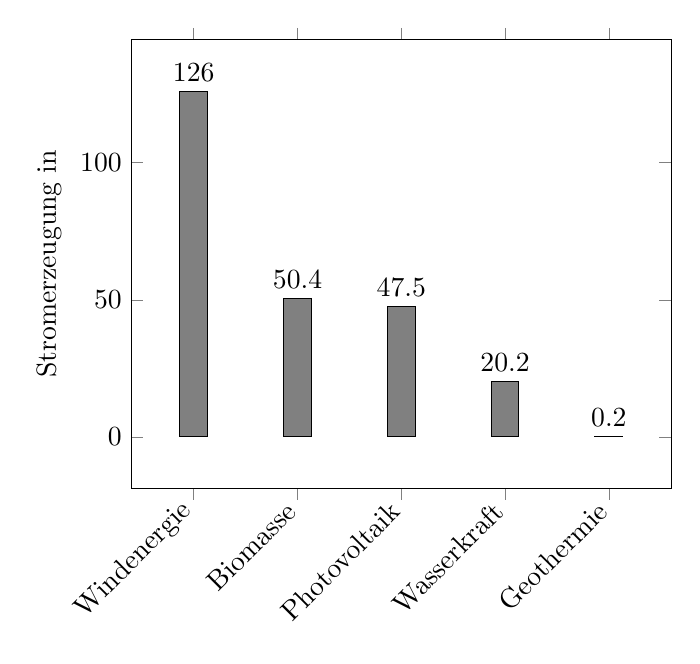
\begin{tikzpicture}
		\begin{axis}[
		ybar,
		enlargelimits=0.15,											% äüßerste bar plots nicht am Limit der x-Achse
		legend style={at={(0.5,-0.2)},
		anchor=north,legend columns=-1},
		ylabel={Stromerzeugung in \SI{}{\twh}},
		symbolic x coords={Windenergie,
			Biomasse,
			Photovoltaik,
			Wasserkraft,
			Geothermie 
		},
		xtick=data,
		nodes near coords,											% Zahlen auf den bar plots
		nodes near coords align={vertical},
		x tick label style={rotate=45,anchor=east},
		]
		\addplot[black,fill=black!50!white] coordinates {
			(Windenergie,126.0) (Biomasse,50.4) (Photovoltaik,47.5)
			(Wasserkraft,20.2) (Geothermie,0.2)
		};
		\end{axis}
	\end{tikzpicture}
	\caption{Verteilung der Bruttostromerzeugung aus erneuerbaren Energien nach Erzeugungsart im Jahr 2019 \parencite{BWE2020}; Eigene Darstellung}
	\label{fig:ee-gen_total}
\end{figure}

Biogasanlagen produzieren mit \SI{29.2}{\twh} den Großteil der Bruttostromerzeugung aus Biomasse, während Biomethan mit einer Erzeugung von \SI{2.7}{\twh} eine untergeordnete Rolle spielt (s. Abb. \ref{fig:ee-gen_biomass}). \parencite{BWE2020} 

% Bar Chart - Biomasse Bruttostromerzeugung 2019

\begin{figure}[H]
	\centering
	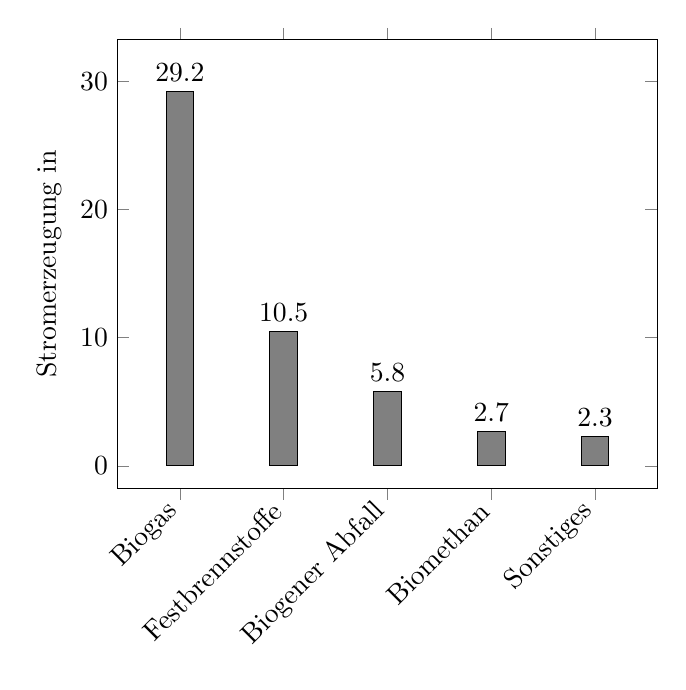
\begin{tikzpicture}
		\begin{axis}[
		ybar,
		enlargelimits=0.15,											% äüßerste bar plots nicht am Limit der x-Achse
		ylabel={Stromerzeugung in \SI{}{\twh}},
		symbolic x coords={Biogas,
			Festbrennstoffe,
			Biogener Abfall,
			Biomethan,
			Sonstiges 
		},
		xtick=data,
		nodes near coords,											% Zahlen auf den bar plots
		nodes near coords align={vertical},
		x tick label style={rotate=45,anchor=east},
		]
		\addplot[black,fill=black!50!white] coordinates {
			(Biogas,29.2) (Festbrennstoffe,10.5) (Biogener Abfall,5.8)
			(Biomethan,2.7) (Sonstiges,2.3)
		};
		\end{axis}
	\end{tikzpicture}
	\caption{Verteilung der Bruttostromerzeugung aus Bioenergie nach Brennstoffart im Jahr 2019 \parencite{BWE2020}; \textit{Eigene Darstellung}}
	\label{fig:ee-gen_biomass}
\end{figure}

Ende 2019 waren in Deutschland mehr als \SI{9000}{\relax} Biogas- und Biomethananlagen mit einer Kraftwerksleistung von \SI{5901}{\mw} bzw. \SI{558}{\mw} am Netz (s. Abb. \ref{fig:ee-cap_biogas}). Seit dem EEG 2012 geht der Zubau von Biogasanlagen deutlich langsamer voran als in den vorangegangenen Jahren. Stattdessen erfolgt aufgrund der Einführung der Flexibilitätsprämie in erster Linie eine Erweiterung bestehender Biogasanlagen, um Flexibilität bereitstellen zu können. \parencite{BWE2020} \parencite{DanielGromke2019}

\begin{figure}[htbp]
	\begin{center}
	\scalebox{0.9}{
	\begin{tikzpicture}
	%%% Bar Plot
	\begin{axis}[
		ybar stacked,
		ymin=-1500,ymax=7000,
		bar width=10pt,
		legend style={
			at={(0.5,-0.20)},
			anchor=east,
			legend columns=1,
			draw=none},
		legend cell align={left},
		ylabel={Leistung in \si{\mega\watt}},
		symbolic x coords={
			2005,
			2006,
			2007,
			2008,
			2009,
			2010,
			2011,
			2012,
			2013,
			2014,
			2015,
			2016,
			2017,
			2018,
			2019
	},
		xtick=data,
		xticklabels={
			2005,,,,,
			2010,,,,,
			2015,,,,
			2019
		},
		%x tick label style={rotate=45,anchor=east},
		ytick={-1000, 0, 1000, 2000, 3000, 4000, 5000, 6000},
		yticklabels={, 0,, 2000,, 4000,, 6000}
		]
	\addplot+[ybar, draw=black, pattern=north east lines] plot coordinates {(2005,665) (2006,1000) (2007,1226) (2008,1419) (2009,2520) (2010,3015) (2011,3837) (2012,4212) (2013,4317) (2014,4380) (2015,4601) (2016,4780) (2017,5173) (2018,5597) (2019,5901) };
	\addplot+[ybar, draw=black, fill=black!50!white] plot coordinates {(2005,0) (2006,0) (2007,6) (2008,16) (2009,18) (2010,96) (2011,218) (2012,256) (2013,383) (2014,603) (2015,614) (2016,653) (2017,567) (2018,557) (2019,558) };
	\legend{\strut Inst. Leistung Biogas, \strut Inst. Leistung Biomethan}
	\end{axis}
	
	%%% Line Plot
	\begin{axis}[
		ymin=-150,ymax=700,
		axis y line*=right,
		legend style={
			at={(0.5,-0.20)},
			anchor=west,
			legend columns=1,
			draw=none},
		legend cell align={left},
		ylabel={Zubau in \si{\mega\watt}},
		symbolic x coords={
			2005,
			2006,
			2007,
			2008,
			2009,
			2010,
			2011,
			2012,
			2013,
			2014,
			2015,
			2016,
			2017,
			2018,
			2019
	},
		xtick=data,
		xticklabels={,,,,,,,,,,,,,,,,,,,,,,,,,,,,,},
		ytick={-100, 0, 100, 200, 300, 400, 500, 600},
		yticklabels={, 0,, 200,, 400,, 600}
		]
	\addplot[sharp plot, draw=black, very thick] plot coordinates {(2005,0) (2006,0) (2007,6) (2008,10) (2009,2) (2010,78) (2011,122) (2012,38) (2013,127) (2014,220) (2015,11) (2016,39) (2017,-86) (2018,-10) (2019,1)};
	\legend{\strut Nettozubau Biomethan}
	\end{axis}
	\end{tikzpicture}
	}
	\caption{Installierte Leistung an Biogas- und Biomethankapazitäten und der Nettozubau von Biomethankapazität \parencite{BWE2020}; Eigene Darstellung}
	\label{fig:ee-gen_total}
	\end{center}
\end{figure}

In den Jahren 2010 bis 2014 gibt es einen verstärkten Ausbau von Biomethananlagen. Ab dem EEG 2014 (s. Kap. \ref{chap:law_theo}) kommt es zu einem starken Einbruch in dem Zubau von Kraftwerksleistung und in den Jahren 2017 und 2018 ist dieser mit einem Rückbau von \SI{86}{\mw} bzw. \SI{10}{\mw} sogar rückläufig (s. Abb. \ref{fig:ee-cap_biogas}). \parencite{BWE2020} Hier zeigt sich die Abschwächung der Anreize seit Neuauflage des EEG 2014.\medskip\\
Insgesamt bedeutet dies, das ein Großteil der bestehenden Anlagenleistung innerhalb des nächsten Jahrzehnts seine Förderung nach dem EEG verlieren wird. Es ist somit dringend geboten alternative Erlösströme zu finden, die über dem Niveau einer reinen Direktvermarktung an der Strombörse liegen, da ansonsten ein Rückgang der Stromerzeugung aus Biogasanlagen zu erwarten ist. Deshalb soll diese Arbeit aufzeigen, ob die Biogasaufbereitung zu Biomethan eine solche Möglichkeit darstellen kann.

% Wie viel kann man an der Strombörse verdienen?

\subsubsection{Verkehr}

Mit einem Endenergieverbrauch von \SI{660}{\gwh} Biomethan im Verkehrssektor im Jahr 2019 ist der Anteil am Gesamtmarkt heute sehr gering. \parencite{BWE2020} Zukünftig kann Biomethan in Form von Bio-\gls{LNG} im Schwerlast-, Schiffs- und Flugverkehr eine bedeutendere Rolle übernehmen, da voraussichtlich Verbrennungsmotoren für lange Zeit die dominierende Antriebstechnologie bleiben werden. \parencite{dena2017}

\subsubsection{Wärme und Kälte}
